\documentclass[aspectratio=169,11pt]{beamer}

\usetheme{Madrid}
\usecolortheme{seahorse}
\setbeameroption{hide notes}
\setbeamercolor{background canvas}{bg=white}
\setbeamercolor{palette primary}{bg=orange!55,fg=black}
\setbeamercolor{palette secondary}{bg=orange!40,fg=black}
\setbeamercolor{palette tertiary}{bg=orange!65,fg=black}
\setbeamercolor{palette quaternary}{bg=orange!32,fg=black}
\setbeamercolor{frametitle}{bg=orange!18,fg=black}
\setbeamercolor{title}{fg=black}
\setbeamercolor{structure}{fg=black}
\setbeamertemplate{footline}[frame number]
\setbeamertemplate{navigation symbols}{}

\usepackage{amsmath}
\usepackage{booktabs}
\usepackage{graphicx}

\title{The Role of Permutation Invariance in Linear Mode Connectivity of Neural Networks}
\author{Entezari et al., ICLR 2022}
\date{}

\newcommand{\paperpage}[2][]{%
  \includegraphics[page=#2,width=\linewidth,#1]{2110.06296v2_rep.pdf}%
}

\begin{document}

\begin{frame}
  \titlepage
  \vspace{-0.3cm}
  \begin{block}{Guiding Question}
    Are different SGD solutions really in different basins?
  \end{block}
  \vfill
  \begin{center}
    {\footnotesize Maciek Lodzinski}
  \end{center}
  \note{
    \begin{itemize}
      \item This talk focuses on loss landscape geometry and linear mode connectivity.
      \item Main claim: after accounting for permutation invariance, many SGD solutions may lie in one basin.
    \end{itemize}
  }
\end{frame}

\begin{frame}{Main Question of the Paper}

\centering
\Large
Are different SGD solutions in different \textbf{basins} --- \\
or in one basin if \textbf{permutation invariance} is taken into account?

\vspace{0.5cm}

\normalsize
\centering
One-Basin Modulo Permutation Hypothesis

\end{frame}

\begin{frame}{What Is a Mode and a Basin in the Loss Landscape?}
  \begin{columns}[T,onlytextwidth]
    \begin{column}{0.54\textwidth}
      \vspace{0.2cm}
      \begin{itemize}
        \item A neural network as a vector $\theta \in \mathbb{R}^{d}$
        \item Each weight is one coordinate
        \item Entire network is one point in $d$-dimensional parameter space
        \item Gradient is equall to 0
        \item Basin as a connected region of low loss around a mode
      \end{itemize}
    \end{column}
    \begin{column}{0.46\textwidth}
      \begin{center}
        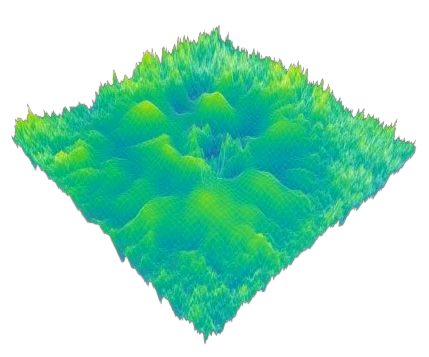
\includegraphics[width=\linewidth,height=0.58\textheight,keepaspectratio]{land.png}
        {\scriptsize \mbox{Example of a loss landscape with multiple minima}}
      \end{center}
    \end{column}
  \end{columns}
  \note{
    \begin{itemize}
      \item Define a mode geometrically before discussing connectivity.
      \item Emphasize that training searches this high-dimensional parameter space.
    \end{itemize}
  }
\end{frame}

\begin{frame}{What Is Linear Mode Connectivity (LMC)?}
  \begin{itemize}
    \item Two trained solutions: $\theta_0,\theta_1$
    \item Linear interpolation:
    \[
      \theta(\lambda)=(1-\lambda)\theta_0+\lambda\theta_1,\quad \lambda\in[0,1]
    \]
    \item Barrier:
    \[
      \max_\lambda \mathcal{L}(\theta(\lambda))-\frac{\mathcal{L}(\theta_0)+\mathcal{L}(\theta_1)}{2}
    \]
    \item Small barrier $\Rightarrow$ same basin under linear path
  \end{itemize}
  \note{
    \begin{itemize}
      \item LMC asks whether a straight line between two solutions stays low loss.
      \item Nonlinear low-loss paths were known; this work explains why linear paths still show barriers.
    \end{itemize}
  }
\end{frame}

\begin{frame}{Permutation Invariance}
  For a hidden-layer permutation matrix $P$:
  \[
    f(x)=W_2\sigma(W_1x)=(W_2P^{-1})\,\sigma(PW_1x).
  \]
  \vspace{0.25cm}

  \begin{itemize}
    \item The function is identical
    \item Different points in parameter space
    \item Creates an artificial barrier between functionally equivalent modes
  \end{itemize}
  \note{
    \begin{itemize}
      \item This is the key intuition behind the conjecture.
      \item The barrier can be viewed as a coordinate-system problem.
    \end{itemize}
  }
\end{frame}

\begin{frame}{Main Conjecture and What It Predicts}
  Let $\mathcal{P}$ be the set of valid hidden-layer permutations. For most SGD solutions $\theta_0,\theta_1$:
  \[
    \exists \pi\in\mathcal{P}\ \text{s.t.}\ 
    \operatorname{Barrier}\!\left(\theta_0,\pi(\theta_1)\right)\approx 0.
  \]
  \vspace{0.15cm}
  \begin{itemize}
    \item Barrier should drop after alignment.
    \item Much of basin multiplicity is representational, not functional.
    \item Only one basin modulo permutation symmetry.
  \end{itemize}
  \vfill
  \begin{center}
    {\large\textit{Are different SGD solutions in different basins --- or in one basin if permutation invariance is taken into account?}}
  \end{center}
  \note{
    \begin{itemize}
      \item This combines the formal claim with the most testable predictions.
      \item If these predictions fail systematically, the conjecture weakens.
    \end{itemize}
  }
\end{frame}

\begin{frame}{Why This Matters}
  \begin{itemize}
    \item \textbf{Federated Learning} — clients train on private data, share only weights; alignment enables averaging making the model better than any individual
        \begin{itemize}
          \item You want to train a model on data from multiple hospitals.
          \item Hospitals can't share patient data, but can share model weights.
          \item Averaged model is better than any individual model, but only if the models are aligned.
        \end{itemize}
    \item \textbf{Efficient Ensembling} — sample diverse models along low-loss paths instead of training multiple networks from scratch
    \item \textbf{Loss Landscape Geometry} — if one basin exists, stochasticity doesn't matter and all SGD solutions are fundamentally equivalent up to symmetry
  \end{itemize}
  \note{
    \begin{itemize}
      \item Not just a geometry question; this determines whether simple model arithmetic is valid.
      \item The central operational claim is: alignment can turn a bad merge into a good one.
      \item Federated learning: hospitals can't share patient data, but can share model weights.
      \item Model Soups (Wortsman et al., 2022) showed averaging fine-tuned models improves accuracy—but relies on shared initialization.
    \end{itemize}
  }
\end{frame}


\begin{frame}{Permuted Modes Experiment}
  \begin{center}
    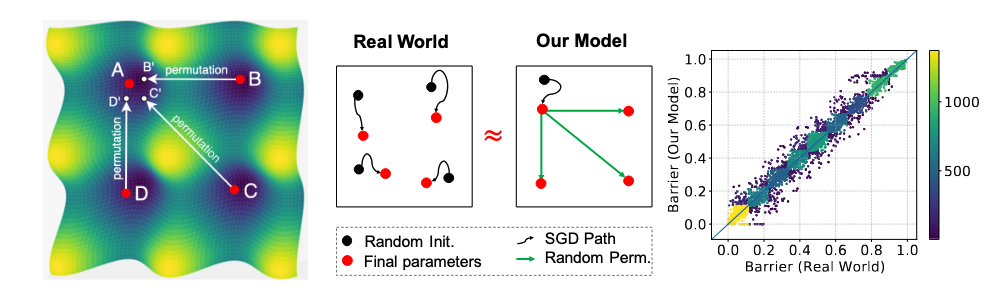
\includegraphics[width=0.95\linewidth,height=0.72\textheight,keepaspectratio]{image.png}
  \end{center}
  \vspace{-0.2cm}
  \centering
  {\scriptsize \textbf{Left:} Permuting neurons can eliminate barriers while preserving function. \textbf{Middle:} The conjecture models independently trained networks as random permutations of the same underlying solution. \textbf{Right:} Barrier distributions between independent networks match those between random permutations.}
  \note{
    \begin{itemize}
      \item This visual replaces Figure 1 and should be used to motivate the same argument.
      \item The interpretation stays the same: many barriers come from mismatch of neuron ordering.
    \end{itemize}
  }
\end{frame}



\begin{frame}{Intractable Search Space}
  \begin{itemize}
    \item Goal: find a permutation that minimizes the interpolation barrier.
    \item Exact search is intractable: for width $n$, one layer already has $n!$ permutations.
    \item Multi-layer networks multiply this combinatorial cost across layers.
  \end{itemize}

  \vspace{0.2cm}
  \textbf{Even small widths explode combinatorially:}
  \begin{itemize}
    \item $8! = 40{,}320$
    \item $16! \approx 2.09 \times 10^{13}$
    \item $32! \approx 2.63 \times 10^{35}$
    \item $64! \approx 1.27 \times 10^{89}$
    \item Two hidden layers with 64 units: $(64!)^2 \approx 1.61 \times 10^{178}$
  \end{itemize}
  \note{
    \begin{itemize}
      \item This motivates why exhaustive search is impossible even for moderate widths.
      \item Combinatorics is the main reason an approximate method is required.
    \end{itemize}
  }
\end{frame}

\begin{frame}{Simulated Annealing}
  \begin{itemize}
    \item Start from an initial permutation (e.g., identity).
    \item Propose a small random change (e.g., swap two neurons).
    \item Accept if barrier decreases.
    \item Otherwise accept with probability $\exp(-\Delta/T)$.
    \item Gradually decrease temperature $T$: exploration first, refinement later.
  \end{itemize}
  \vfill
  \begin{center}
    \footnotesize
    Example proposal (swap two entries):\\[0.2em]
    $\pi = [1,2,3,4,5,6,7,8] \rightarrow \pi' = [1,2,7,4,5,6,3,8]$\\
    (swap positions 3 and 7)
  \end{center}
  \note{
    \begin{itemize}
      \item SA is a tractable heuristic, not a guarantee of globally optimal permutation.
      \item This directly leads to the SA results shown on the next slide.
    \end{itemize}
  }
\end{frame}


\begin{frame}{Results of the SA Algorithm}
  \begin{center}
    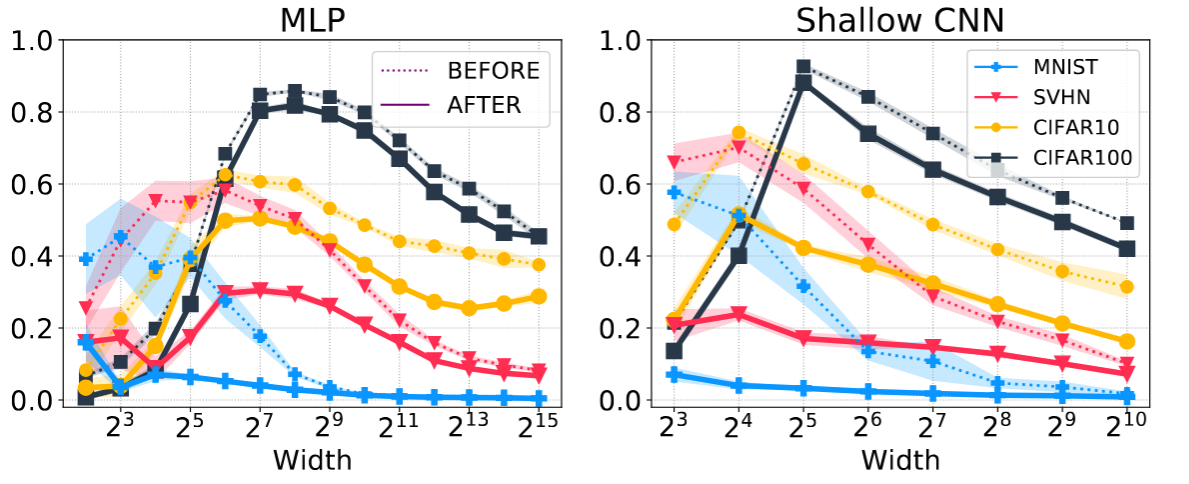
\includegraphics[width=0.93\linewidth,height=0.56\textheight,keepaspectratio]{anneal.png}
  \end{center}
  \vspace{-0.2cm}
  \centering
  {\scriptsize We take two SGD solutions $\theta_1$ and $\theta_2$, permute $\theta_1$, and report the barrier between permuted $\theta_1$ and $\theta_2$ as found by SA.}
  \vspace{0.1cm}
  \footnotesize
  \begin{itemize}
    \item SA finds permutations that \textbf{lower the barrier}.
    \item The barrier usually does \textbf{not} drop to 0.
    \item Ambiguity remains: this can mean either genuinely different basins or a weak permutation-finding method.
  \end{itemize}
  \note{
    \begin{itemize}
      \item Highlight the key limitation: reduced barrier is evidence for symmetry, but non-zero barrier is not conclusive.
      \item This is a method-versus-hypothesis identifiability issue.
    \end{itemize}
  }
\end{frame}

\begin{frame}{Where the Conjecture Is Supported and Where It Is Lacking}
  \begin{itemize}
    \item \textcolor{green!60!black}{\textbf{$\checkmark$}} Two wide one-hidden-layer NNs at initialization can be aligned via permutation.
    \item \textcolor{green!60!black}{\textbf{$\checkmark$}} Similarity between barriers for different trained modes and for a mode versus its permuted version.
    \item \textcolor{green!60!black}{\textbf{$\checkmark$}} Approximate permutation search lowers the barrier.
    \item \textcolor{red!75!black}{\textbf{$\times$}} Still no full proof for deep networks.
    \item \textcolor{red!75!black}{\textbf{$\times$}} No perfect alignment method, so non-zero barriers are inconclusive.
    \item \textcolor{red!75!black}{\textbf{$\times$}} Permutation alligning of already permuted mode experiment is inherently flawed.
  \end{itemize}
  \note{
    \begin{itemize}
      \item First three are supporting evidence; last two are current limitations.
      \item This keeps the support-versus-gap distinction explicit.
    \end{itemize}
  }
\end{frame}

\begin{frame}{My Thesis in Context of Linear Mode Connectivity and Permutation Invariance Paper}
  \vspace{1em}
  \textbf{This thesis asks:}
  \begin{itemize}
    \item Are there any easily findable counterexamples to the one-basin modulo permutation hypothesis?
    \item Can we develop permutation-finding method that achieve lower barriers?
    \item What changes if we correct the flawed experiment by permuting a shifted version of a mode instead?
  \end{itemize}
  
  \note{
    \begin{itemize}
      \item Entezari et al. provided statistical evidence but no constructive proof.
      \item Git Re-Basin later showed permutations can be found for wide networks.
      \item It fails on VGG and narrow networks; this may be method failure or hypothesis failure.
      \item My contribution: controlled experiments to distinguish these cases.
    \end{itemize}
  }
\end{frame}



\end{document}
